\documentclass{report}
\title{\Large  Physics 20 - Differential Equations}
\author{\large Shubh Agrawal, \normalsize\emph{Class of 2022}}
\date{\small November 4, 2018}
\usepackage[a4paper,top=2cm, left=2.5cm,width=13cm,bottom=2cm,right=2.5cm]{geometry}
\usepackage{amsthm, amsmath, amssymb, tipa, graphicx, caption, subcaption, float, fancyhdr, graphics}

\pagestyle{fancy}
\lhead{Shubh Agrawal}
\rhead{Physics 20}
\chead{Differential Equations}

\begin{document}
\maketitle
\section*{Part 1}
The initial conditions were taken such that the block-spring system is supposed to be at maximum displacement (taken as unity, for simplification of calculations) and minimum velocity (zero, from static observer reference). So, $x_0=1$ and $v_0=0$ for the entire discussion in this report.
\subsection*{Explicit Method}
\subsubsection*{Numerical Spring Model}
Linear space plots of $x$-versus-$t$ and $v$-versus-$t$ were simulated for different  $h$ (small change value) to find a suitable value for the rest of discussion. The number of iterations $N$ was varied such that the number of  oscillations simulated was constant. 
\begin{figure}[H]
	\centering
	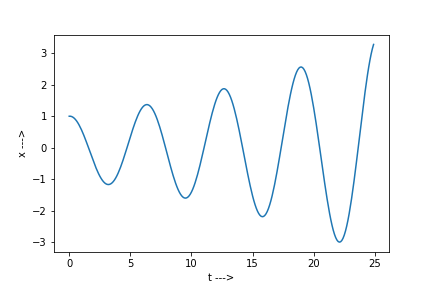
\includegraphics[width = 0.8\textwidth]{tXeA.png}
	\label{tXeA}
	\caption{Position $x$ as a function of time $t$ simulated by numerical spring at $h=0.1$, $N=250$, giving nearly 4 oscillations. Note that the deviation of amplitude ($\propto\sigma$) from 1 grows to 200\%.}
\end{figure}
\begin{figure}[H]
	\centering
	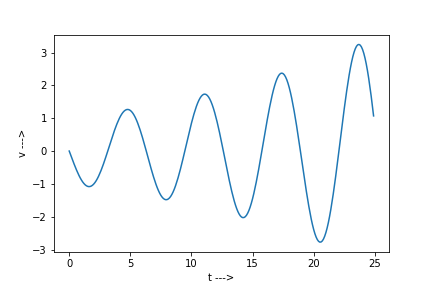
\includegraphics[width = 0.8\textwidth]{tVeA.png}
	\label{tVeA}
	\caption{Velocity $x$ as a function of time $t$ simulated by numerical spring at $h=0.1$, $N=250$. Again, note that the deviation of maximum velocity ($\propto\sigma$) from 1 grows to 200\% over four oscillations.}
\end{figure}
\begin{figure}[H]
	\centering
	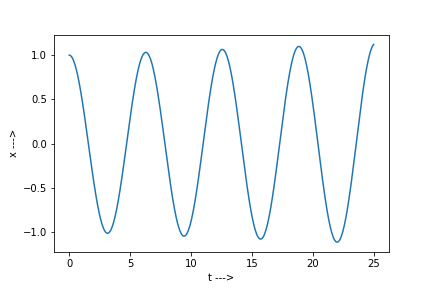
\includegraphics[width = 0.8\textwidth]{tXe.png}
	\label{tXe}
	\caption{Position $x$ as a function of time $t$ simulated by numerical spring at $h=0.01$, $N=2500$, giving nearly 4 oscillations. It is noted that this simulation is more stable for our domain.}
\end{figure}
\begin{figure}[H]
	\centering
	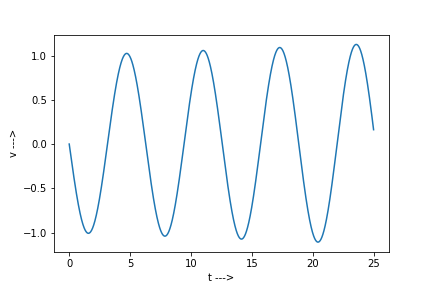
\includegraphics[width = 0.8\textwidth]{tVe.png}
	\label{tVe}
	\caption{Velocity $v$ as a function of time $t$ simulated by numerical spring at $h=0.01$, $N=2500$, giving nearly 4 oscillations. }
\end{figure}
The latter two simulations are reasonably fast (graphs were produced in under a second) and are sufficiently accurate ($\sigma$ is less than 20\%), but still show deviations which are to be studied. So, for the rest of discussion and comparison, the values $h=0.01$ and $N=2500$ would be used.\\
It is notable that in all of these explicit method models, the amplitude and maximum velocity increase over time (that is, iterations of recursive model).
\subsubsection*{Comparison to Analytical spring}
We know that $F=ma$, and for this system, $F=-kx$. Also note that $a= \frac{d}{dt}v=\frac{d^2}{dt^2}x$. To find the real solutions to the spring setup, we must solve the differential equation:
$$\frac{d^2x}{dt^2}=-\frac{k}{m}x$$
which has the solution of form $x = A_x \sin(\omega t)$. Now, we have set up $x_0= A_x=1$ (as $v_0=0$) and $\omega = k/m = 1$. Also, using $\frac{dx}{dt}=v$, the solution analytically is derived to be:
\begin{align*}
	x &= \sin t\\
    v &= \cos t
\end{align*}
Using these, the plots of instantaneous errors are plotted against time (number of simulations).
\begin{figure}[H]
	\centering
	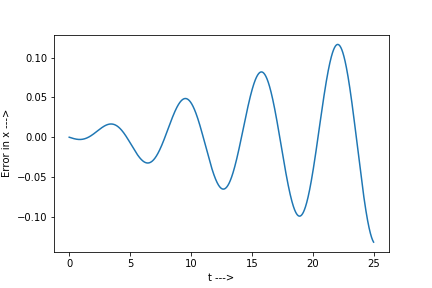
\includegraphics[width = 0.8\textwidth]{eXe.png}
	\label{errorinXe}
	\caption{Linear space plot of error in position value $x$ as a function of time, with $h=0.01$, $N=2500$. Note that error is oscillatory and magnitude of maximum error increases with time. Also note that error is out of phase from $x$ with $\Delta\phi =\pi/2$, and in phase with $v$. }
\end{figure}
\begin{figure}[H]
	\centering
	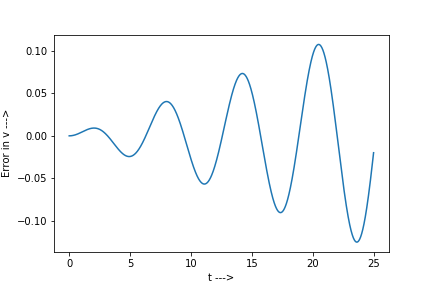
\includegraphics[width = 0.8\textwidth]{eVe.png}
	\label{errorinVe}
	\caption{Linear space plot of error in velocity value v as a function of time, with $h=0.01$, $N=2500$. Note that error is oscillatory and magnitude of maximum error increases with time. Also note that error is out of phase from $v$ with $\Delta\phi =\pi$.}
\end{figure}
\subsubsection*{Truncation error}
Models were run for geometrically decreasing values of $h$, that is, for $h=h_0, \frac{h_0}{2}, \frac{h_0}{4}, \frac{h_0}{8}, \frac{h_0}{16}$ ($N$ was scaled accordingly). In the first two graphs of this section denoting the global error progression with time, these models are represented by \emph{blue, orange, green, pink,} and \emph{purple} respectively. The maximum value of error attained during these simulations was taken as the truncation error.
\begin{figure}[H]
	\centering
	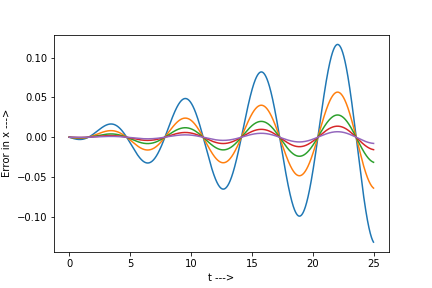
\includegraphics[width = 0.8\textwidth]{eXc.png}
	\label{trXe}
	\caption{Errors in $x$ as a function of time for varying coefficient $h$. Note that by decreasing increment value and increasing the number of total simulations (iterations), more accurate models are obtained from the explicit numerical spring.}
\end{figure}
\begin{figure}[H]
	\centering
	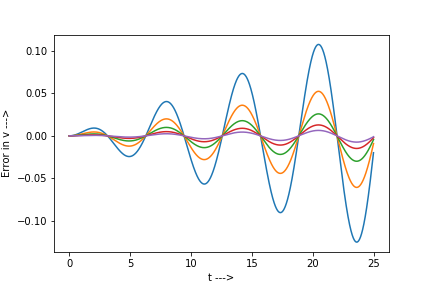
\includegraphics[width = 0.8\textwidth]{eVc.png}
	\label{trVe}
	\caption{Errors in $v$ as a function of time for geometrically varying coefficient $h$. Note that by decreasing increment value and generating more iterations, accuracy of velocity models increases too.}
\end{figure}
\begin{figure}[H]
	\centering
	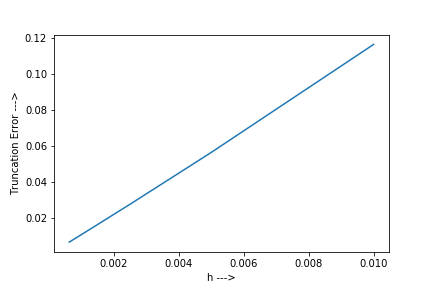
\includegraphics[width = 0.8\textwidth]{trE.png}
	\label{logloge}
	\caption{Linear space plot of truncation error against the increment/decrement coefficient $h$. Note that, even with just five data points, the graph is reasonably linear. The straight line relation shows the direct proportionality of truncation error to $h$.}
\end{figure}

\subsubsection*{Time dependency of normalized Energy}
Note that the value of normalized total energy must be constant in an non-dissipative system (which we have here, ideally), and would be equal to the initial value $x_0^2 + v_0^2 = 1$.
\begin{figure}[H]
	\centering
	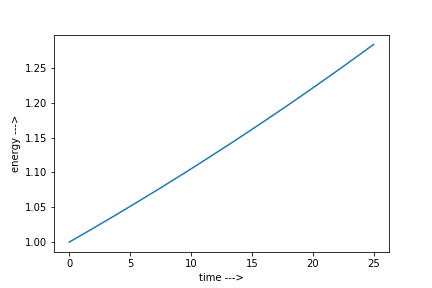
\includegraphics[width = 0.8\textwidth]{energye1.png}
	\label{en1e}
	\caption{Total energy as a function against time (or number of iterations) for $h=0.01$, $N=2500$. Note that energy which should be conserved shows a deviation of over 25\% in just four oscillations. Worth noting is the fact that in spite of being a non-ideal numeric model, the rules still give a linear plot, instead of a oscillating curve.}
\end{figure}
\begin{figure}[H]
	\centering
	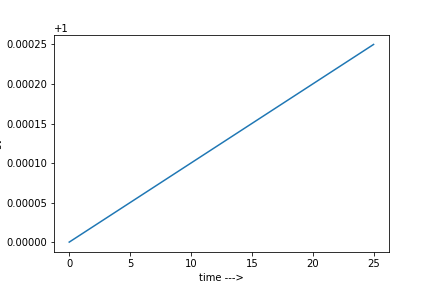
\includegraphics[width = 0.8\textwidth]{energye2.png}
	\label{en2e}
	\caption{Total energy as a function against time (or number of iterations) for $h=0.0001$, $N=2500000$. This model took a considerably longer time to run (~20 seconds), and still an error of 0.025\% is seen in just four cycles, in a quantity which should be ideally conserved.}
\end{figure}

\subsection*{Implicit Method (and comparison with Explicit Method)}
This section includes plots for the implicit method under similar conditions as that of the previous section. An important inclusion is plots comparing the model outputs under both set of rules.
\subsubsection*{Numerical Spring Model}
\begin{figure}[H]
	\centering
	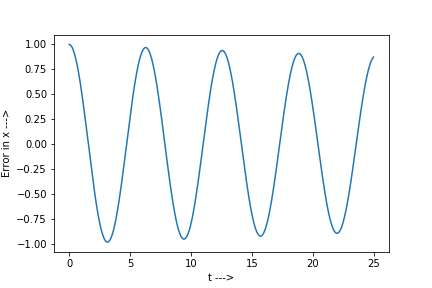
\includegraphics[width = 0.8\textwidth]{tXi.png}
	\label{tXi}
	\caption{Position $x$ as a function of time $t$ simulated by numerical spring at $h=0.01$, $N=2500$, giving nearly 4 oscillations. Note that under this model, the amplitude of oscillations progressively decreases.}
\end{figure}
\begin{figure}[H]
	\centering
	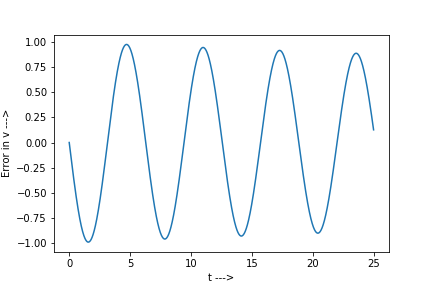
\includegraphics[width = 0.8\textwidth]{tVi.png}
	\label{tVi}
	\caption{Velocity $v$ as a function of time $t$ simulated by numerical spring at $h=0.01$, $N=2500$, giving nearly 4 oscillations. Note that velocity amplitude is decreasing with time.}
\end{figure}
\begin{figure}[H]
	\centering
	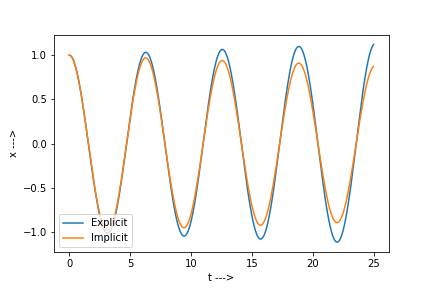
\includegraphics[width = 0.8\textwidth]{cx.png}
	\label{cx}
	\caption{Overlayed plots of position $x$ against time ($\propto$iterations) under both explicit and implicit methods.Note that the explicit values for amplitude increase from the initial of 1, while the implicit amplitude values go below 1.}
\end{figure}
\begin{figure}[H]
	\centering
	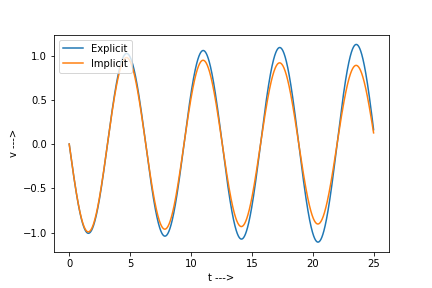
\includegraphics[width = 0.8\textwidth]{cv.png}
	\label{cv}
	\caption{Overlayed plots of velocity $v$ against time or number of iterations.  Note that nature of error is opposite between the two.}
\end{figure}
\subsubsection*{Comparison to Analytical spring}
We use the same analytical solutions as before to compare the numeric spring generated by the implicit method.
\begin{align*}
x &= \sin t\\
v &= \cos t
\end{align*}
\begin{figure}[H]
	\centering
	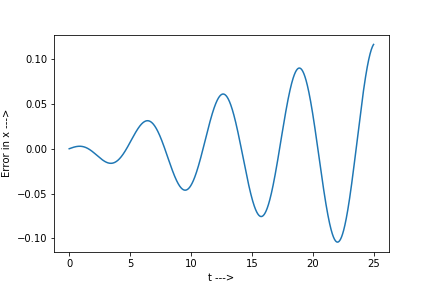
\includegraphics[width = 0.8\textwidth]{eXi.png}
	\label{eXi}
	\caption{Linear space plot of error in position value $x$ as a function of time, with $h=0.01$, $N=2500$. Note that error is oscillatory and magnitude of maximum error increases with time. Also note that error is out of phase from $x$ with $\Delta\phi =- \pi/2$, and in inverse phase with $v$ ($\Delta\phi = \pi$).}
\end{figure}
\begin{figure}[H]
	\centering
	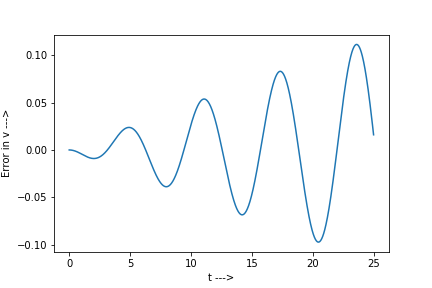
\includegraphics[width = 0.8\textwidth]{eVi.png}
	\label{eVi}
	\caption{Linear space plot of velocity global error against time, with $h=0.01$, $N=2500$. Note that error is oscillatory and magnitude of maximum error increases with time. Also note that error is in phase with $v$.}
\end{figure}
\begin{figure}[H]
	\centering
	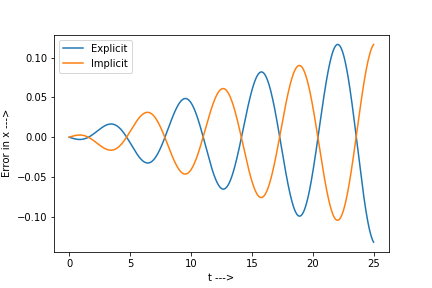
\includegraphics[width = 0.8\textwidth]{cex.png}
	\label{cex}
	\caption{Overlayed plots of positional global errors against time $t$ (number of simulations). Note that the magnitudes of errors are similar with respect to time, but opposite in sign: the two oscillatory waves are out of phase with half-cycle difference ($\Delta\phi = \pi$).}
\end{figure}
\begin{figure}[H]
	\centering
	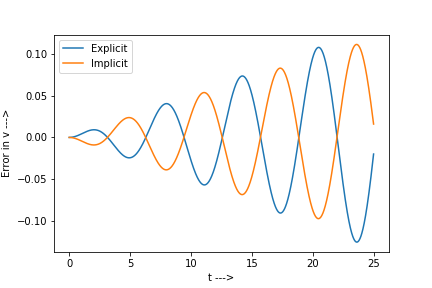
\includegraphics[width = 0.8\textwidth]{cev.png}
	\label{cev}
	\caption{Overlayed plots of velocity global errors against time $t$ . Note again that the magnitudes of errors are similar at given time, with the two oscillatory curves out of phase at half-cycle difference ($\Delta\phi = \pi$).}
\end{figure}
\subsubsection*{Truncation error}
As earlier, models were run for geometrically decreasing values of $h$, that is, for $h=h_0, \frac{h_0}{2}, \frac{h_0}{4}, \frac{h_0}{8}, \frac{h_0}{16}$ ($N$ being scaled accordingly)- represented by \emph{blue, orange, green, pink,} and \emph{purple} respectively.
\begin{figure}[H]
	\centering
	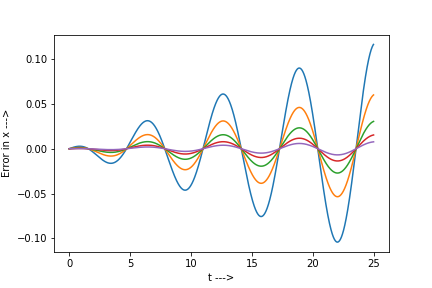
\includegraphics[width = 0.8\textwidth]{eXci.png}
	\label{trXi}
	\caption{Overlayed liner space plots of positional error as predicted by the implicit method for various $h$, against time (number of recursive iterations). Note that for all five values of $h$, the graphs are in the same phase (in sync). The error for smaller steps/larger numbr of simulations is, as expected, lower.}
\end{figure}
\begin{figure}[H]
	\centering
	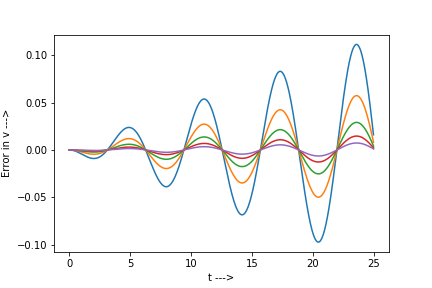
\includegraphics[width = 0.8\textwidth]{eVci.png}
	\label{trVi}
	\caption{Errors in $v$ as a function of time for geometrically varying coefficient $h$. Note that by decreasing increment value and generating more iterations, accuracy of velocity models increases too.}
\end{figure}
\begin{figure}[H]
	\centering
	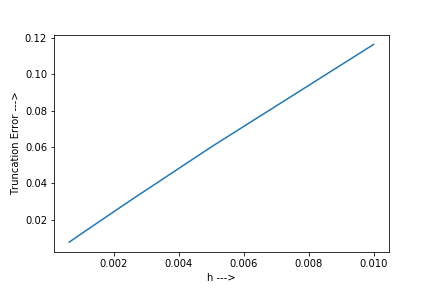
\includegraphics[width = 0.8\textwidth]{trI.png}
	\label{loglogi}
	\caption{Linear space plot of truncation error (maximum x-based error) against the step coefficient $h$. Note that the graph is reasonably linear. The straight line relation shows the direct proportionality of truncation error to $h$, as we had in the explicit method.}
\end{figure}
\begin{figure}[H]
	\centering
	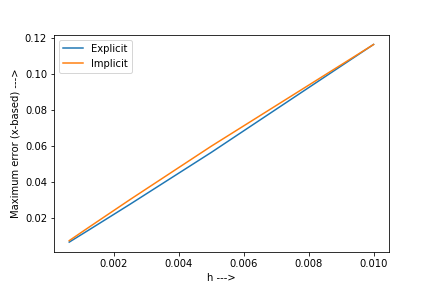
\includegraphics[width = 0.8\textwidth]{trC.png}
	\label{compareTR}
	\caption{Overlayed truncation error-step coefficient $h$ plots for explicit and implicit models of numeric spring. Note that the two plots fairly overlap, notably given the end points overlap and the plots are supposed to be straight lines. The slight disjoint in the middle portion can be attributed to the fact that the order of magnitude of $h$ is still high ($\geq-3$) and we have only 5 data-points for either line.}
\end{figure}

\subsubsection*{Time dependency of normalized Energy}
The normalized total energy of this isolated system should again be constant ideally, and equal to initial value of $x_0^2 + v_0^2 = 1$.
\begin{figure}[H]
	\centering
	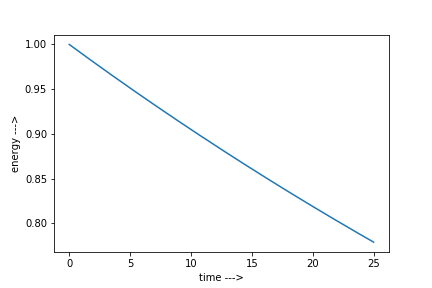
\includegraphics[width = 0.8\textwidth]{energyi1.png}
	\label{en1i}
	\caption{Total energy as a function against time (or number of iterations) for $h=0.01$, $N=2500$. Note that energy, which should be ideally conserved, shows a deviation of over 20\% in just under four oscillations. Also note that the predicted energy of system decreases, as expected from the known fact that predicted $x$ and $v$ amplitudes are decreasing.}
\end{figure}
\begin{figure}[H]
	\centering
	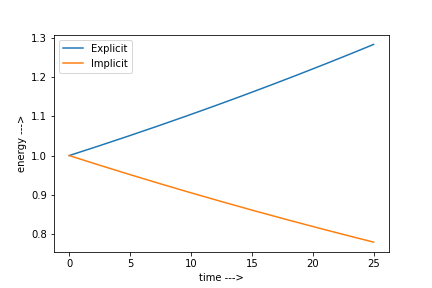
\includegraphics[width = 0.8\textwidth]{compareE.png}
	\label{bothen}
	\caption{Temporal evolution of total system energy as predicted by explicit and implicit methods. Note that, while starting at the same initial value, the explicit prediction increases and the implicit value decrease. Note that the deviation of the latter (~20\%) is less than the former (~25\%), showing that implicit method is favorable when energy analysis is a dominant factor. This behavior may be attributed to the fact that while explicit predications can diverge to infinity, the implicit simulation's energy must still remain greater than zero; so the magnitude of slope of curve decreases- thus, yielding a lower overall decrease (=deviation)}
\end{figure}

\pagebreak

\section*{Part 2}
\subsection*{Phase Space Geometry}
For each of these simulations, while step size coefficient was kept the same as earlier analysis ($h=0.01$), the number of simulations was appropriately changed to produce more readable plots (In a way that while the starting point is on the X- axis $(1.0,0.0)$, the end of curve is distinctly distinguishable from any point on the axes.). As $E=x^2 + v^2$ is ideally conserved, so $x$-$v$ plots are analytically circles: any deviations point to the existence and nature of errors.
\subsubsection*{Explicit Method}
\begin{figure}[H]
	\centering
	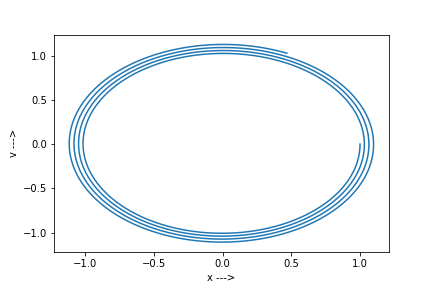
\includegraphics[width = 0.8\textwidth]{phaseE.png}
	\label{pE1}
	\caption{Linear space plot of position against velocity for an explicit method simulation for $h=0.01$, $N=2400$. Note that this curve is open and clockwise, with an increasing radius. This is expected as the energy of the system (as predicted numerically), which is the square of the radius, increases with each subsequent simulation.}
\end{figure}
\begin{figure}[H]
	\centering
	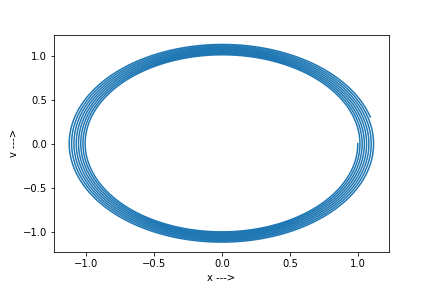
\includegraphics[width = 0.8\textwidth]{phaseE2.png}
	\label{pE2}
	\caption{Linear space plot of position against velocity for an explicit method simulation for $h=0.005$, $N=10000$. Note that even after increasing the number of iterations and decreasing the interval gaps, the increase in radius is still observed, and a open shape is obtained.}
\end{figure}
\subsubsection*{Implicit Method}
\begin{figure}[H]
	\centering
	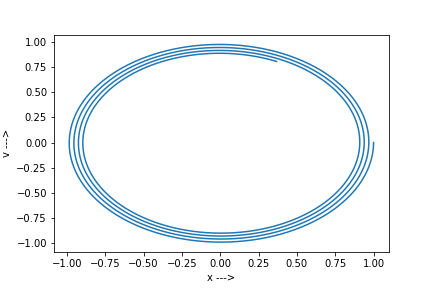
\includegraphics[width = 0.8\textwidth]{phasei1.png}
	\label{pI}
	\caption{Linear space plot of position against velocity for an implicit method simulation for $h=0.01$, $N=2400$. Note that this curve is open and clockwise, with an decreasing radius. This is expected as the energy of the system (as predicted numerically) decreases with each iteration.}
\end{figure}
\begin{figure}[H]
	\centering
	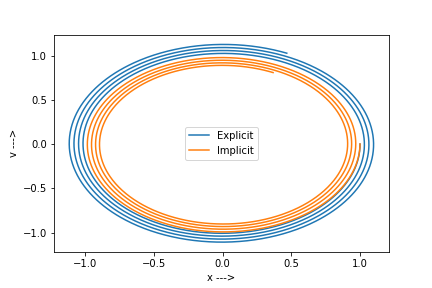
\includegraphics[width = 0.8\textwidth]{compared.png}
	\label{comEI}
	\caption{Overlayed $x$-$v$ plots for explicit and implicit methods. Note that the initial point and direction of curve (clockwise) is same for each curve, as expected, but they spiral differently - outward and inward respectively.}
\end{figure}
\subsubsection*{Symplectic Euler method}
\begin{figure}[H]
	\centering
	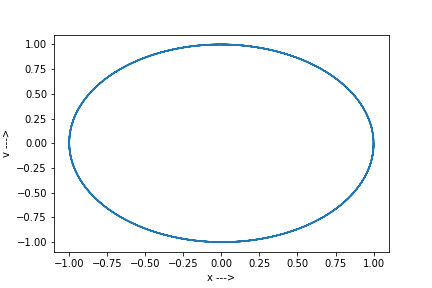
\includegraphics[width = 0.8\textwidth]{euler.png}
	\label{eulerphase}
	\caption{Linear space plot of position against velocity for a symplectic Euler method simulation for $h=0.01$, $N=2400$. Note that the curve does not seem to ``spiral'' inward or outward like the former two do; in fact, it seems to be a closed figure, and a circle. However, it is notable that the curve is not an exact overlap as the line is thicker due to some small differences.}
\end{figure}
\begin{figure}[H]
	\centering
	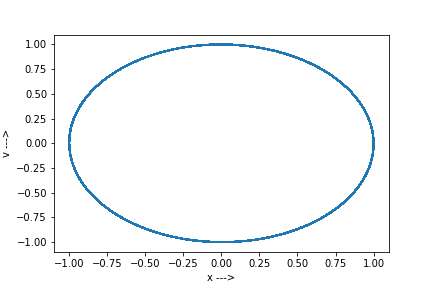
\includegraphics[width = 0.8\textwidth]{euler2.png}
	\label{eulermag}
	\caption{Linear space plot of position against velocity for a symplectic Euler simulation for $h=0.01$, $N= 250000$. As $N$ is now appreciatively large and no change in radius of curve is apparent, it is safe to hypothesize (which would be proved/reasoned with next graph) that the radius does not have an unbounded increase or decrease, and under the rules, it is periodic in some sense.}
\end{figure}
\begin{figure}[H]
	\centering
	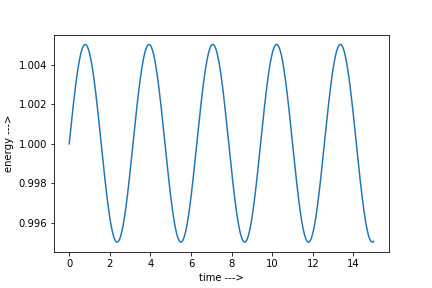
\includegraphics[width = 0.8\textwidth]{eulerEN.png}
	\label{eulerenergy}
	\caption{Temporal (time-dependent) evolution of total system energy as predicted by the symplectic Euler method, with $h=0.01$ and $N=1500$. Note that the energy (which is the square of radius) is, as suspected/hypothesized, periodic and bounded (above \& below). This also explains the minor deviations from the perfect circle in the above two plots. It is also notable that as $h$ would be decreases, the deviations from the ideal constant value would decrease, and thus, the simulation can be reduced to practically a constant energy system, even over very large time (not possible for the other two methods as the errors are monotonic w.r.t. time).}
\end{figure}
\end{document}